% Rangefinding

\chapter{Determining Ranges} % Main chapter title

\label{Rangefinding}

%----------------------------------------------------------------------------------------

This chapter covers the rangefinding subsystem, the part of the project which determines the ranges between two sensors. The ranges are later fed into the position calculation subsystem, which determines the positions of the sensors in 3D space.

This chapter covers three main topics:
\begin{enumerate}
	\item A description of what the rangefinding system does, and the devices composing it.
	\item The math behind calculating the range between two sensors.
	\item A description of the networking protocol developed for this project.
\end{enumerate}

\section{The System}
\begin{figure}
	\centering
	\tikzstyle{vertex}=[circle, draw]
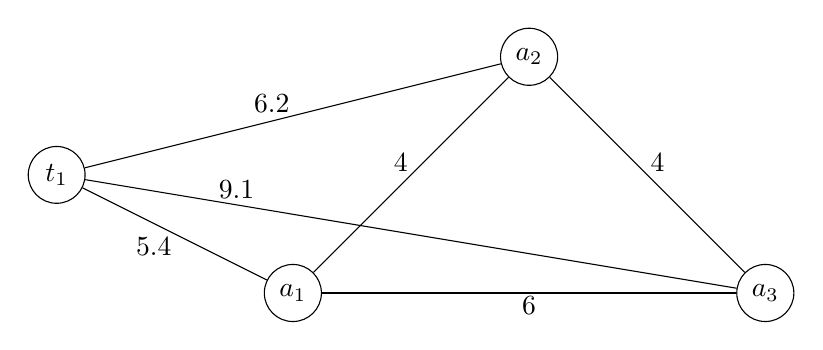
\begin{tikzpicture}[transform shape]
\node[vertex](a1) at (0, 0) {$ a_1 $};
\node[vertex](a2) at (3, 3) {$ a_2 $};
\node[vertex](a3) at (6, 0) {$ a_3 $};
\node[vertex](t1) at (-3,1.5) {$ t_1 $};

\begin{scope}[every path/.style={-}, every node/.style={inner sep=1pt}]
       \draw (a1) -- node [anchor=south east] {$4$} (a2);
       \draw (a2) -- node [anchor=south west] {$4$} (a3);
       \draw (a1) -- node [anchor=north] {$6$} (a3);
       \draw (t1) -- node [anchor=north east] {$5.4$} (a1);
       \draw (t1) -- node [anchor=south east] {$6.2$} (a2);
       \draw (t1) -- node [pos=0.2, anchor=south west] {$9.1$} (a3);
\end{scope} 
\end{tikzpicture}
	\decoRule
	\caption{An example network, showing 1 tag $t_1$ and 3 anchors $a_i$ and the reported distances between them. Note that each device calculates its own range to the other devices, which will be slightly different from the range calculated on the other devices. This is not shown on the diagram.}
	\label{fig:ExampleNetwork}
\end{figure}

The rangefinding subsystem is comprised of \textbf{nodes} in a network, each of which is capable of sending and receiving wireless signals.

Each node is either an \textbf{anchor} or a \textbf{tag}. Both tags and anchors use essentially the same hardware and code, but anchors are assumed to be stationary while tags are mobile. Stationary nodes are required so as to provide a consistent frame of reference for other nodes when calculating positions later on. More information on this can be found in Section~\ref{FrameOfReference}.

The rangefinding subsystem's purpose is to determine the distances between every pair of nodes in the network. With this data, the position calculation subsystem can then determine the positions of every anchor and tag in 3D space. An example 2D rangefinding network is shown in Figure~\ref{fig:ExampleNetwork}.

\section{Rangefinding}
Rangefinding is the act of determining the distance between two things. Rangefinding is done wirelessly. The underlying concept is that if we precisely note the times at which we send and receive a signal, then -- since light travels at a fixed speed -- we can determine the distance the signal traveled, which is the distance between the nodes. 

The basic algorithm for the network is: 
\begin{enumerate}
	\item Each node broadcasts a message to every other node, and every node responds. 
	\item The time it took for the message to travel from one node to another and then back (minus the time spent processing the received messages) is calculated.
	\item With some simple math involving the speed of light the distance between the nodes is calculated. 
\end{enumerate}

This method of calculating range is known as \textbf{time-of-flight} (TOF).

Each node is comprised of a DWM1000, can send wireless signals, and an Arduino microcontroller.

\section{Requirements}
The scope of the project is to handle precise rangefinding indoors in a room. The requirements for the system were:
\begin{itemize}
	\item The system must be able to produce ranges accurate to within three meters or less that are not noisy (regular swings of $\pm$ one meter would be unacceptable). Otherwise, what was displayed in the augmented reality portion of the project would not be useful. 
	\item The system must calculate ranges at frequencies greater than 3Hz. Otherwise, moving objects will have their positions displayed inaccurately (and the system would be misleading).
	\item The system must be able to rangefind within an area the size of a room (at least 5x5 meters). 
	\item The system must be able to robustly handle nodes entering and leaving the network. 
\end{itemize}

It will be demonstrated how we sought to satisfy these criteria.

\section{Time-of-Flight}
This section briefly covers the math behind time-of-flight range calculations. For more in-depth information, \textcite{DW1000UserManual} has a comprehensive write-up of the different ways wireless ranging can be performed as well as an error analysis.

\subsection{Propagation Time}
The goal behind time-of-flight is to measure the propagation time of a signal, $T_{prop}$. Once we obtain this, it is a simple measure to calculate the distance $d$ between the two nodes using the speed of light, $c$, with the following formula:

\[
	d = c T_{prop}
\] 

\subsection{Single-sided Two-Way Ranging}
\begin{figure}
	\centering
	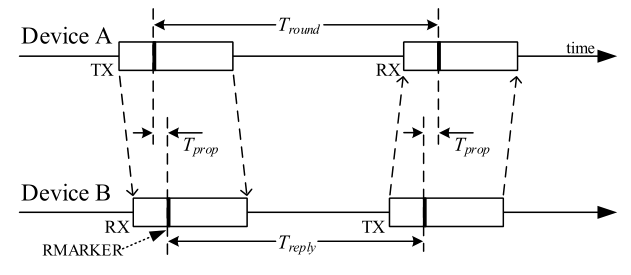
\includegraphics[width=\linewidth]{Figures/BasicRanging.png}
	\decoRule
	\caption{Single-sided two-way ranging \cite{DW1000UserManual}.}
	\label{fig:BasicRanging}
\end{figure}

In the case where there are two nodes communicating with each other, \parencite{DW1000UserManual} states that one can calculate the time it takes a signal to propagate between them, $T_{prop}$, as:

\[
	T_{prop} = \frac{T_{round} - T_{reply}}{2}
\]

where $T_{round}$ and $T_{process}$ are the total durations between receiving and transmitting messages as can be seen in Figure~\ref{fig:BasicRanging}.

\subsection{Double-sided Two-way Ranging}

\begin{figure}
	\centering
	\includegraphics[width=\linewidth]{Figures/AsyncRanging.png}
	\decoRule
	\caption{Double-sided two-way ranging with three messages \cite{DW1000UserManual}.}
	\label{fig:AsyncRanging}
\end{figure}

Because the clocks of two nodes may not pass time at the same rate (clock skew), the above equation will suffer from significant error. This is because processing times far dwarf the time it takes a signal to propagate. \parencite{DW1000UserManual} presents, without proof, the following equation for more accurate rangefinding:

\[
	T_{prop} = \frac{T_{round1}  T_{round2} - T_{reply1} T_{reply2}}{T_{round1} + T_{round2} + T_{reply1} + T_{reply2}}
\]

where $T_{round1}$, $T_{round2}$, $T_{reply1}$, $T_{reply2}$ are the durations between sending and receiving messages as seen in Figure~\ref{fig:AsyncRanging}. An independently derived proof of this equation can be found in Appendix~\ref{AsyncProof}.

Because the ranging has two rounds, after the initial calculation of range we can calculate a new range value for every single following transmission by re-using the last timestamps received for the beginning of the next round.

\section{Networking Basics}

Each node in the network broadcasts in a round robin fashion, with a small break after each node has transmitted. As part of the transmitted message, the node transmits the timestamp of when it is sending the message, a list of the timestamps when it last received a communication from every other node in the network, and a list of the last computed ranges to the other nodes. Every other node in the network will receive this information and use it to compute a new range to the node in question. Thus, every node in the network receives complete range information for the whole network.

The DWM uses 40 bits (5 bytes) for its timestamps. The Arduino internally represents these as 64-bit integers (the last byte being meaninless), but transmits them as 40 bit (5 byte) numbers.

Every node in the network has a pre-determined ID, which is set when it the code is programmed onto the device. A single byte is used for this ID to save as much space as possible, though the code could easily be modified to support longer IDs if the devices were to be mass produced. Alternately, something like DHCP could be implemented. As there are only 7 devices currently operational, our project only uses IDs 1 through 7, though the IDs do need not be consecutive. ID 255 is a special dummy value used in the code and should not be selected for use with an actual device.

Communications between the Arduino and the DWM1000 are handled through SPI. When the DWM1000 receives a message, it triggers an interrupt on the Arduino, which can then obtain the received data through SPI.

\section{Communications Timing}

\begin{figure}
	\centering
	\begin{tikzpicture}

\def \n {6}
\def \radius {3cm}
\def \margin {11} % margin in angles, depends on the radius

\begin{scope}[auto, every node/.style={draw,circle,minimum size=2em,inner sep=1},node distance=2cm]
\foreach \id [count=\s] in {1, 2, 5, 8, 10, 255}
{
  \node at ({360/\n * (\s - 1)}:\radius) {$\id$};
  \draw[->, >=latex] ({360/\n * (\s - 1)+\margin}:\radius) 
    arc ({360/\n * (\s - 1)+\margin}:{360/\n * (\s)-\margin}:\radius);
}
\end{scope}

\end{tikzpicture}
	\decoRule
	\caption{Transmission order of a network composed of five devices with IDs 1, 2, 5, 8, and 10. Note they transmit in order, and there is a dummy ID of 255 which serves as a marker for the end of the round.}
	\label{fig:TransmissionOrder}
\end{figure}

In order to maximize the operating frequency of the system and provide as smooth a visual experience as possible on the phone, we want to minimize the amount of time a node is not transmitting. In order to do this, it was decided that nodes should transmit in order of their ID in a round robin fashion. A round of transmissions are performed, each node transmitting once, and then it repeats. When one node receives a transmission, it checks to see if it is its turn and then transmits as soon as it can.

This round robin ordering is done by creating an ordered array of IDs in the network. When a transmission is received, the network increments the index of the next expected device to transmit by one. A device can tell whether it should transmit by checking to see if its ID is equal to the ID of the next expected node to transmit. If so, it transmits. 

The downside to this approach is that if any transmission were to be lost, for example by interference or electrical noise, the network would grind to a halt as it waits for a message that is never going to come. A solution to this is to include a timer that tracks a window in which a message should be received. If it takes too long to receive a message, the device was assumed to have to failed to transmit for some reason and the next device will take their turn and transmit.

To help the network be more robust, for example if one node has a clock that runs faster than the others (making it think a transmission is late when it is not), the network assumes whatever device last transmitted was right in doing so, and sets the index of the next node to transmit in the ordered array as being one higher than it.

This approach also raises the question of how new nodes will join the network if a node is constantly transmitting. To solve this, a small delay is added at the end of each round. When a device wishes to enter the network, it waits for the end of a round, and then does a transmission in this added space. This transmission lets all devices know it is part of the network, and they will add it to their ordered lists of IDs appropriately. 

In the code, this delay at the end of the round is implemented by adding a dummy node with the ID of 255 (the highest ID possible with one byte) to the network. The nodes will wait for a transmission from it at the end of each round, but it will never come, at which point the round starts over with the lowest ID transmitting. An example ordering can be found in Figure~\ref{fig:TransmissionOrder}.

An unsolved issue here is what happens when the transmission to join the network is sent and it is not received. This will cause the joining device to have a wrong order, and it will transmit at the same time as another device every round. Since the chances of this happening are quite low and could be solved by resetting the joining device, this is not dealt with. A possible solution to deal with this would be having the receiving device check the responses of all the other nodes to make sure they all received its transmission, and, if they have not, then to retransmit in the space at the end of the round until they do.

Code for this logic can be found in the \code{loop} function of Appendix~\ref{ArduinoCode}.

\section{Range Information Protocol}
\begin{figure}
	\centering
	\usetikzlibrary{calc,positioning,shapes,decorations.pathreplacing}

% the styles for short and long nodes
\tikzset{
short/.style={draw,rectangle,minimum height=1.5cm,
  text width=7pt,align=center,fill=gray!30, text centered},
long/.style={short,text width=1.9cm}
}

% the short nodes \shnode{<label>}{<right of>}{<text>}
\def\shnode#1#2#3{%
  \node[short,right=of #1] (#2) {\rotatebox{270}{#3}}}

% the long nodes \lnode{<label>}{<right of>}
\def\lnode#1#2#3#4{%
  \node[long,right=of #1,label={below:#4}] (#2) {#3}}
  
 \def\idnode#1#2#3#4{%
  \node[short,right=of #1,label={below:#4},style={short,text width=1.1cm}] (#2) {#3}}

\noindent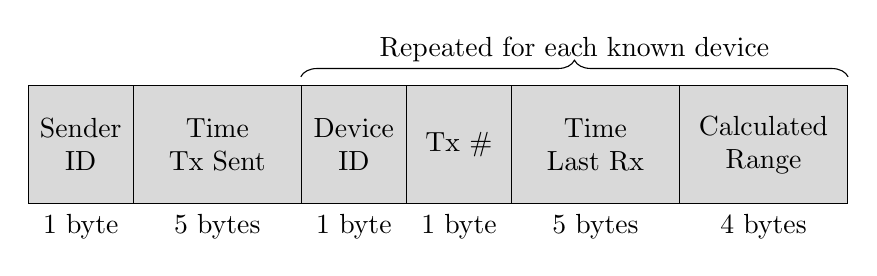
\begin{tikzpicture}[node distance=-\pgflinewidth]

\node[short,label={below:1 byte},style={short,text width=1.1cm}] (a) {Sender ID};
\lnode{a}{b}{Time Tx Sent}{5 bytes};
\idnode{b}{c}{Device ID}{1 byte};
\idnode{c}{d}{Tx \#}{1 byte};
\lnode{d}{e}{Time Last Rx}{5 bytes};
\lnode{e}{f}{Calculated Range}{4 bytes};

\draw[decorate,decoration={brace,raise=3pt,amplitude=0.6em}] (c.north west) -- node[above=5pt] {Repeated for each known device} (f.north east);

\end{tikzpicture}
	\decoRule
	\caption{Data packet diagram for the rangefinding network.}
	\label{fig:NetworkPacket}
\end{figure}

The protocol for a transmission from a node is as follows:

\begin{itemize}
	\item 1 byte for the ID of the transmitting node. The ID cannot not be 255.
	\item 5 bytes for the timestamp of the sending of the message.
	\item For each device the transmitting node has knowledge of:
	\begin{itemize}
		\item 1 byte for the ID of the device.
		\item 1 byte for a shared transmission counter. This counter is incremented by one whenever a message is received, and also incremented when one is sent. If a message is received or sent and the transmission counter on the device does not match the counter in the message, a transmission was lost. The message is thrown away and the transmission counter set to 0 to let the other device know there was an error on the next transmission.
		\item 5 bytes for timestamp of last received message from the device.
		\item 4 bytes for last calculated range to that device. Note that the two devices will each calculate slightly different ranges to each other.
	\end{itemize} 
\end{itemize}

Parsing a received message and updating range values from the parsed data is fairly straightforward. The code in question can be found in the \texttt{parseReceived} function in Appendix \ref{ArduinoCode}.

\section{Summary}
todo



